\documentclass[12pt]{article}
%\usepackage{report}

\usepackage[utf8]{inputenc} % allow utf-8 input
%\usepackage[T1]{fontenc}    % use 8-bit T1 fonts
\usepackage[colorlinks=true, linkcolor=blue, citecolor=blue, urlcolor=blue]{hyperref}       % hyperlinks
\usepackage{url}            % simple URL typesetting
\usepackage{booktabs}       % professional-quality tables
\usepackage{amsfonts}       % blackboard math symbols
\usepackage{nicefrac}       % compact symbols for 1/2, etc.
%\usepackage{microtype}      % microtypography
\usepackage{lipsum}		% Can be removed after putting your text content
\usepackage{graphicx}
\usepackage{footnote}
\usepackage{doi}
\usepackage{comment}
\usepackage{multirow}
\usepackage{textcomp}
\usepackage{gensymb}
\usepackage{float}
\usepackage{amsmath}
%\usepackage{subfigure}
\usepackage{subcaption}
\usepackage{setspace}
\usepackage[skip=10pt plus1pt]{parskip} 
\usepackage[top=3cm, bottom=3cm, left=2.5cm, right=2.5cm]{geometry}
\usepackage{titlesec}
\begin{document}
\onehalfspacing
\begin{titlepage}
    \centering
    
\includegraphics[width=3cm]{crest.jpg}\par
    \vspace{0.3cm}
    {\scshape\Large School of Mathematical Sciences \par}
    \vspace{0.25cm}
    {\scshape\Large The University of Southampton \par}
    \vspace{0.25cm}
    {\Large MATH 6149 - Modelling with Differential Equations \par}
    \vspace{0.5cm}
    {\huge\bfseries Flash Floods!\par}
    \vspace{0.5cm}

    {\Large Chin Phin Ong (Linus) \par}
    \vspace{0.25cm}
    {\large Student ID: 33184747 \par}
    {\large  \par}
    \vfill
    {\large February 2025 \par}
\end{titlepage}

\begin{abstract}
    Flash floods are dangerous and unpredictable, caused by rapid flooding after intense rainfall, often within a few hours. In this study, we develop a mathematical model to describe flash flood dynamics using first-order hyperbolic PDEs based on mass and momentum conservation. We consider different river cross sections — rectangular, wedge-shaped, semicircular, and parabolic — and derive the corresponding perimeter and flux expressions. The formation and evolution of shocks are analysed using characteristic diagrams, providing insight into how rapid changes in flow develop. Numerical solutions are computed using Godunov's method, which effectively handles shock formation due to non-linear wave propagation. The model is tested under realistic rainfall conditions, showing how river geometry influences the behaviour of flood waves.
\end{abstract}

\section{Introduction}
Flash floods are dangerous phenomena characterized by rapid flooding, typically within 3 to 6 hours after heavy rainfall \cite{national-oceanic-and-atmospheric-administration-no-date}. In this short study, the mathematics behind flash flooding will be investigated. We will attempt to model the behaviour of flash floods using differential equations. Following that, the characteristic diagrams (Section \ref{sec:characteristic}) are presented for different initial conditions for different cross sections.

\section{Modelling}
To start, we will take a section of a river bed of length $s$, where the cross section of the river that is filled with water at time $t$ is $A(s, t)$, the cross section's perimeter of the riverbed that comes into contact with water is $l(s, t)$, and the angle of slope of the riverbed is $\alpha$. 

Let's start by writing an equation to model the flow of water. We can start with a simple conservation law: water flowing in = water flowing out, since  water is incompressible and we make the assumption that water is not evaporated into the surroundings, nor is it absorbed by the riverbed and it does not  have any external sources of water. Considering a thin slice of the river, we can write the infinitesimal volume, $dS$ in between $s$ and $s + ds$:
\begin{equation}
    dV = A(s,t)ds
\end{equation}

If flow of water into the cross section is denoted as the flux, $Q(s, t)$, the flow of water out is $Q(s +  ds, t)$. The rate of change of volume of water can be written as:
\begin{align}
    \frac{d}{dt}(dV) &= Q(s,t) - Q(s+ds,t) \approx -\frac{\partial Q}{\partial s}(s,t)ds, \\
    &\implies \frac{\partial A(s,t)}{\partial t}ds \approx -\frac{\partial Q}{\partial s}(s,t)ds.
    \\ &\implies \frac{\partial A}{\partial t} + \frac{\partial Q}{\partial s} =0. \label{PDE general}
\end{align}

The flux can be written in terms of the cross sectional area and the area averaged velocity, $\bar{u}(s, t)$ as:
\begin{equation}
    Q(s,t) = A(s, t) \bar{u}(s, t)
    \label{eqn:qAu}
\end{equation}

The drag of turbulent flows have been measured experimentally and it has been concluded that the shear stress, $\tau$ (friction force per unite area, opposite in direction to flow) on the walls of a channel is:
\begin{equation}
    \tau = f \rho \bar{u}^2
\end{equation}
Where $\rho$ is the density of water and $f$ is the friction factor that is dependant on the walls and the geometry of the channel. The frictional and gravitational force between for an infinitesimally small section $s$ and $s + ds$ is:
\begin{equation}
    \begin{split}
        dF_{friction} &= \tau l(A)ds
        \\dF_{gravity} &= g\sin{\alpha}\rho A ds
    \end{split}
\end{equation}
Assuming that there is no external force required to accelerate the flow, we can equate the gravitational and frictional forces, giving:
\begin{equation}
    \begin{split}
        \tau=&\frac{g\sin{\alpha}\rho A}{l(A)}=f\rho\bar{u}^2
       \\ \implies&\bar{u}= \sqrt{\frac{g\sin{(\alpha)A}}{l(A)}}
    \end{split}
\end{equation}

Rewriting equation \ref{PDE general} using \ref{eqn:qAu} and substituting our expression of $\bar{u}$, we end up with the first order hyperbolic PDE for $A$.
\begin{equation}
\label{PDE_of_A}
\boxed{\qquad
    \frac{\partial A}{\partial t} + \sqrt{\frac{g}{f}} \frac{\partial}{\partial s}\left(A^{\frac{3}{2}}\sqrt{\frac{\sin \alpha}{l (A)}}\right) = 0 \qquad
    }
\end{equation}

Where $\alpha$ is the angle of inclination of the river bed, where the values will be obtained from \cite{ROSGEN1994169}. We will explore different cross sections and the relationship of the perimeter, $l(A)$ on the cross sectional area $A$ will also be stated, and Eqn. \ref{PDE_of_A} will be solved.

%%insert figure of different cross sections here
\begin{figure}[ht]
    \centering
    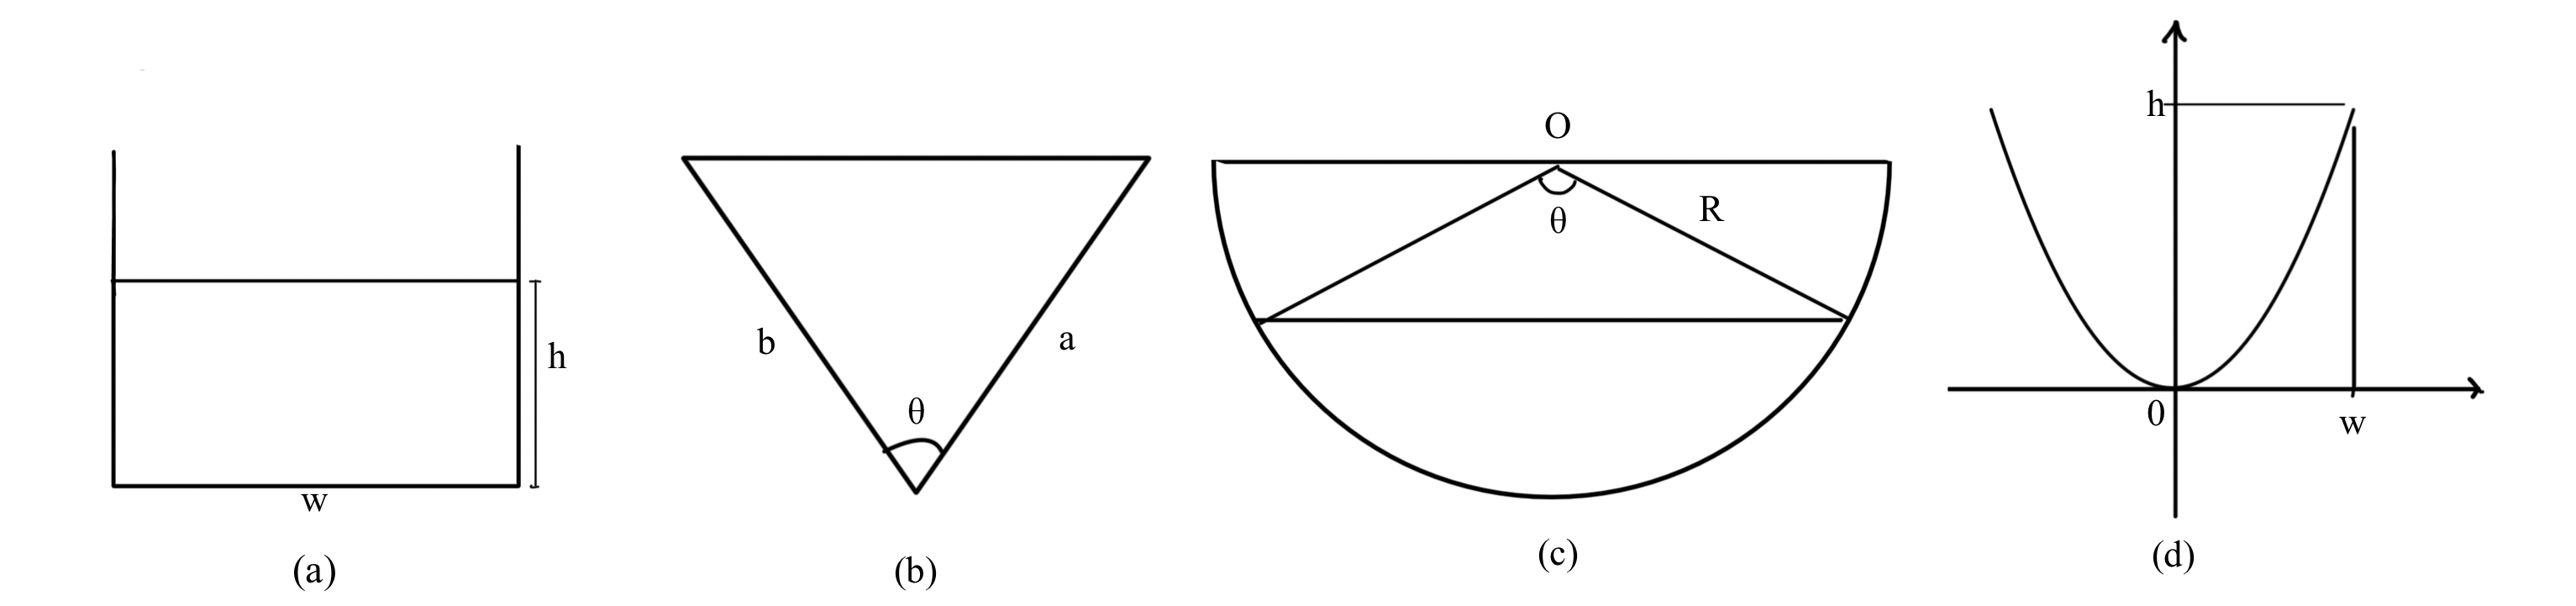
\includegraphics[width=
\linewidth]{Figures/cross_sections.jpeg}
    \caption{Types of cross sections of rivers, the types that will be considered in this paper. (a) Rectangle, (b) Wedge, (c) Semi-circle, (d) Parabola.}
    \label{fig:cross-sections}
\end{figure}

\section{Characteristic Diagrams}
\label{sec:characteristic}
We can attempt to solve the equation numerically. One of the many ways is to visualise the solutions to the equation using characteristic diagrams. A characteristic diagram is used as a graphical representation to solutions of a hyperbolic PDE (i.e. Eqn. \ref{PDE_of_A}). Characteristic diagrams help visualize how solutions propagate in time and space, usually in the $(s, t)$ plane, where $s$ and $t$ is the spatial and time coordinate respectively. Characteristic curves trace the evolution of points in the solution, with their slopes corresponding to the wave speed at each point. Intersections of these curves indicate the formation of shocks, which correspond to discontinuities in the solution.

We can compare Eqn. \ref{PDE_of_A} with the following PDE:
\begin{equation}
    \frac{\partial A}{\partial t} + v(A) \frac{\partial A}{\partial s} = 0\qquad 
\end{equation}
Where $v(A)$ is now known as the wave speed which at which disturbances propagate in the system and is the slope, that depends on A. The solution propagates along characteristic curves in the $(s, t)$ plane. Moreover, we can see that: 
\begin{equation}
    \begin{split}
        a \frac{\partial f(A)}{\partial s} &= v(A)\frac{\partial A}{\partial s}
        \\ v(A)  &= a \frac{\partial f(A)}{\partial s}\frac{\partial s}{\partial A}
        \\ &= a \frac{\partial f(A)}{\partial A} \qquad \text{where }a\text{ is a constant}
    \end{split}
\end{equation}
We can derive a general formula for the wave speed.
\begin{equation}
    \begin{split}
        v(A) &= \sqrt{\frac{g\sin \alpha}{f}}\frac{\partial}{\partial A}\left( \sqrt{\frac{A^3}{l(A)}}\right)
        \\&= \sqrt{\frac{g\sin \alpha}{f}}\frac{\partial}{\partial A}\left(\frac{3}{2}A^{1/2}\cdot l(A)^{1/2}\right)
        \\&= \frac{1}{2}\sqrt{\frac{g\sin \alpha}{f}}\left(3\sqrt{\frac{A}{l(A)}} - {\left(\frac{A}{l(A)}\right)^{3/2}}l'(A) \right)
    \end{split}
\end{equation}

Shock formation occurs when characteristic curves intersect, leading to discontinuities in the solution. Characteristic curves are in the form $ x(s, t) = P(s, 0) + v(A(s))\cdot t$, where $P(s, 0)$ is a different initial point along the spatial axis (in this case, different points in the river). These shocks correspond to rapid changes in flow variables, such as water depth or velocity, and are a fundamental feature of non-linear wave propagation in hydrodynamics. The characteristic curves will be plotted for different values of $P(s, 0)$ in Python. In order to get a shock, initial conditions have to be set. For an initial condition for $A(s, t)$, a Gaussian distribution will be used as to mimic the conditions \textbf{after} a heavy rainfall. The area of rainfall follows the distribution:
\begin{equation}
     A_\text{Rainfall} = \frac{V}{\sqrt{2\pi\sigma^2}}\exp{\left(-\frac{(s - \mu)^2}{\sigma^2}\right)} + A_{initial}
\end{equation}

Where:
\begin{itemize}
    \item $V$ is the volume of rainfall
    \item $s$ is the spatial coordinate along the length of the river
    \item $\mu$ is the mean that corresponds to the point along the river where the majority of rainfall occurs
    \item $\sigma$ is the standard distribution of the rain
\end{itemize}

We should define the constants that are shared between the different cross sections. We require that: $g = 9.81 \text{ ms}^{-2}$), $f = 0.1$, $A_{initial} = $, $\sigma = $, $\mu  = 0$. The non-constant variables will be the angle of the riverbed, $\alpha$ and the various variables that are unique to the different cross sections which will be discussed in Section \ref{sec:results}.

\section{Godunov's Method}
Godunov's method is a numerical method to obtain an accurate solution to a hyperbolic PDE with shocks. In this scheme, we use the Finite Volume Method. We consider the first order hyperbolic PDE of the form:
\begin{equation}
    \frac{\partial c}{\partial t} + \frac{\partial}{\partial x}Q(c) = 0
\end{equation}

Comparing with Eqn. \ref{PDE_of_A}, we can conclude:
\begin{equation}
    \frac{dA_i}{dt} + Q(A_i) - Q(A_{i-1}) = 0 \qquad \text{for} \qquad i = 1, 2, ..., N
\end{equation}
Where:
\begin{equation}
    Q(A) = \sqrt{\frac{g\sin\alpha}{f}}\sqrt{\frac{A^3}{l(A)}}
\end{equation}
This is what is cited in the notes. However, in the actual code I take a different approach. The spatial domain is discretised into cells, where I approximate solutions as piecewise constant. Then I solve the PDE $\frac{\partial c}{\partial t} + \frac{\partial}{\partial x}Q(c) = 0$ at the boundary. One can set the time step, $dt$ to obey the Courant–Friedrichs–Lewy (CFL) conditions \cite{courant1967partial} to ensure stability. We use the upwind scheme such that flux is calculated based on the flow. The cross sectional area is then evaluated by:
\begin{equation}
    A_{new}[i] = A[i] - \frac{dt}{dx}(Q[i + 1] - Q[i])
\end{equation}
And can be visualised in the $(A, s)$ plane by plotting curves of $f(A, s)$ for different values of $t$ to observe time evolution of the state.

\subsection{Shock velocity}
Since the PDE (Eqn. \ref{PDE general}) is from the conservation law (from lecture notes):
\begin{equation}
    \frac{d}{dt}\int_a^b A(s, t)ds + [Q(A(s, t)]_a^b = 0
    \label{eqn:conservation_law_oint}
\end{equation}
One an determine the speed of the shock by picking values $a$ and $b$ close to the shock. This allows the approximation of the integral to be:
\begin{equation}
    \begin{split}
        &\int_a^b A(s, t)ds \approx A_0 (h(t) - a) + A_1(b - h(t))
        \\
    \\ \text{where: }& A_0 = A(s(t)-a, t), \qquad A_1 = A(b - s(t),t)
    \\
    \\ &\frac{d}{dt}\int_a^b A(s, t)ds = \dot s(t)(A_0 - A_1)
    \\ &\boxed{\text{ }\dot s(t) = \frac{Q(A_1)- Q(A_0)}{A_1 - A_0} = \frac{[Q(A)]_{s(t)}}{[A]_{s(t)}}\text{ }}
    \end{split}
\end{equation}

It is important to understand how the shock evolves with time. It is obtained using the shock velocity equation, where  for the first two characteristic curves that intersect$[\cdot]_{s(t)}$ is the jump in values across the shock at $x = s(t)$. $A_1$ and $A_2$ are the areas of the first and second characteristic curves respectively.

\section{Simulations}
\label{sec:results}
The values of $\alpha$ will be obtained from \cite{ROSGEN1994169}. The values of $\alpha$s are in gradient percentage from \cite{ROSGEN1994169}, where the formulae to convert to radians is: $\phi = \arctan{\theta}$, where $\theta$ and $\phi$ are the angles in gradient percentage and radians respectively. We will have a rainfall volume $V = 5,000\text{ m}^3$ \cite{} with a standard deviation $\sigma = 100\text{ m}$. The code that plots the characteristic equations is the function \verb|plot_characteristics| in \verb|characteristic_plot.py|. For the Gudonov method, the file \verb|gudonov.py| is used. The code can be found on GitHub\cite{linsuong_2023}. The objective of this is to observe the evolution of the water in the river, and to test the two methods and see if they line up with each other. Calculation of wave speed is also be done via code.

\subsection{Rectangular Channel}
For the rectangular channel of width $w$ and height of water $h$ (Fig. \ref{fig:cross-sections}), the area and perimeter respectively are: $A = wh$ and $l(A) = w + \frac{2A}{w}$, giving a first order derivative of :$l'(A) = \frac{2}{w}$ (See Appendix \ref{appendix:rectangle} for detailed derivation). Meanwhile, $\alpha = 2\%$ and $w = 10\text{ m}$. Plotting the characteristic diagram gives the plot shown in Fig. \ref{fig:rect_char}.
\begin{figure}[ht]
    \centering
    \begin{subfigure}[b]{0.49\textwidth}
        \centering
        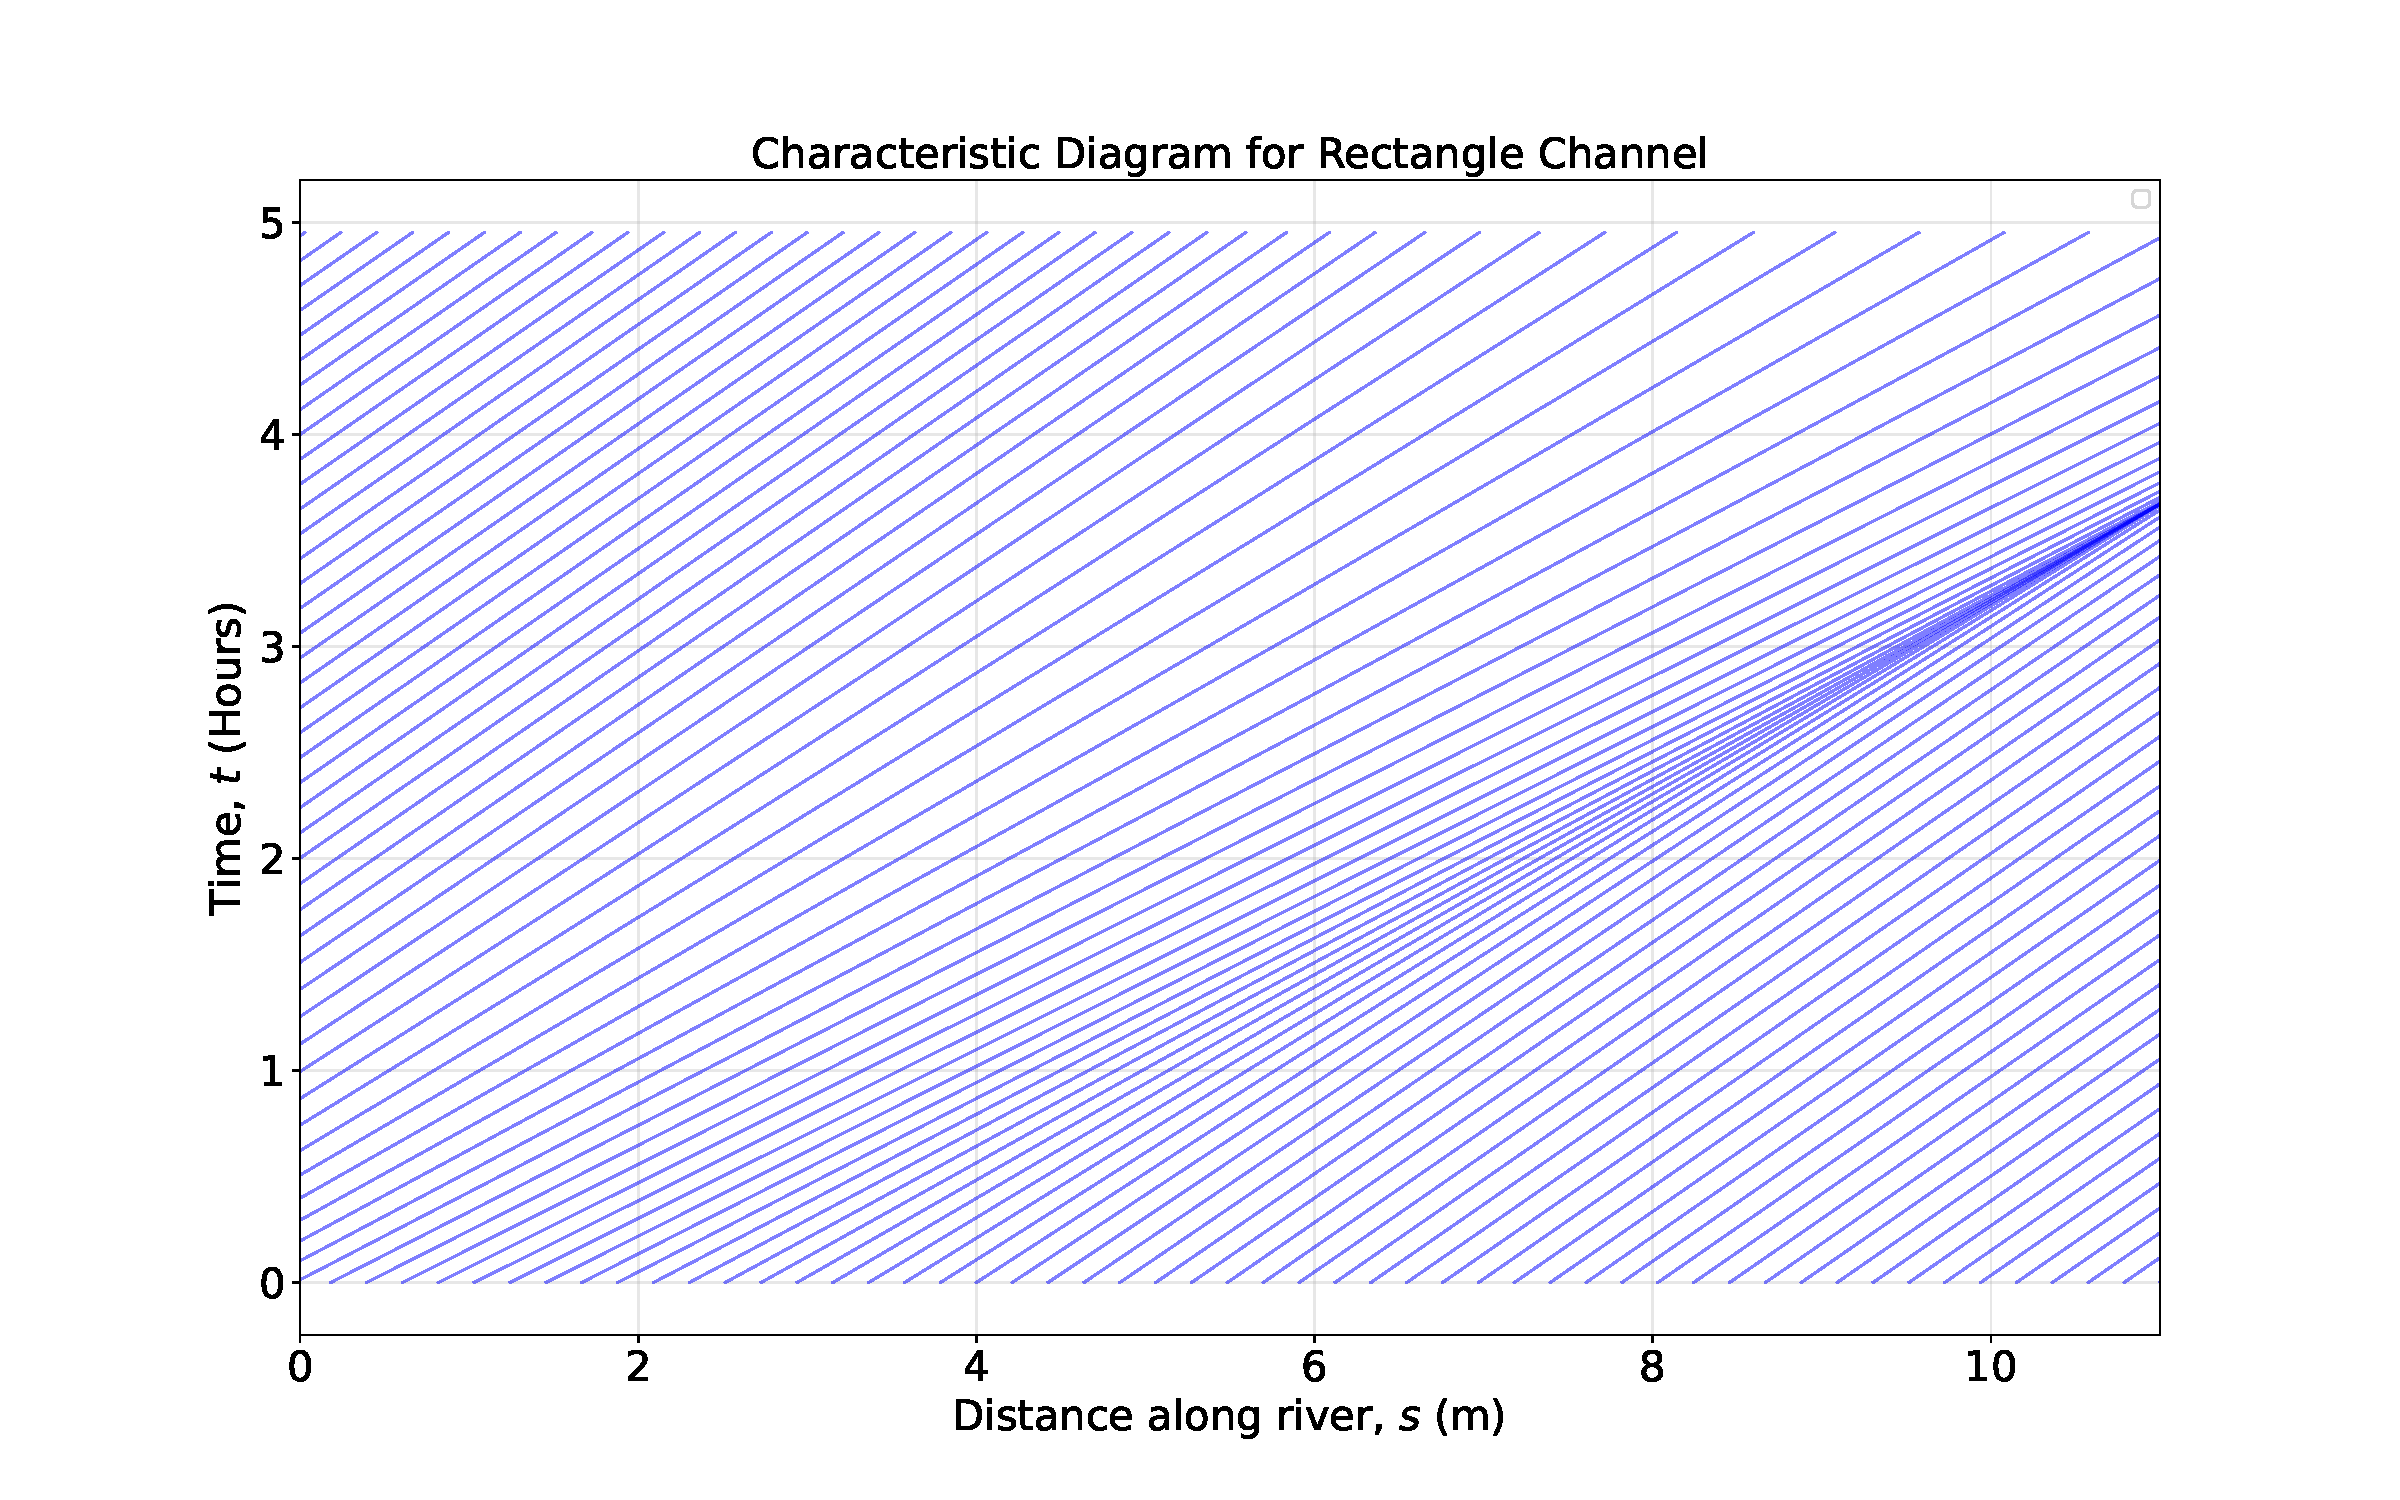
\includegraphics[width=\textwidth]{Figures/Rectangle_characteristic.pdf}
        \caption{Characteristic equations for the rectangular cross sections}
        \label{fig:rect_char}
    \end{subfigure}
    \hfill
    \begin{subfigure}[b]{0.49\textwidth}
        \centering
        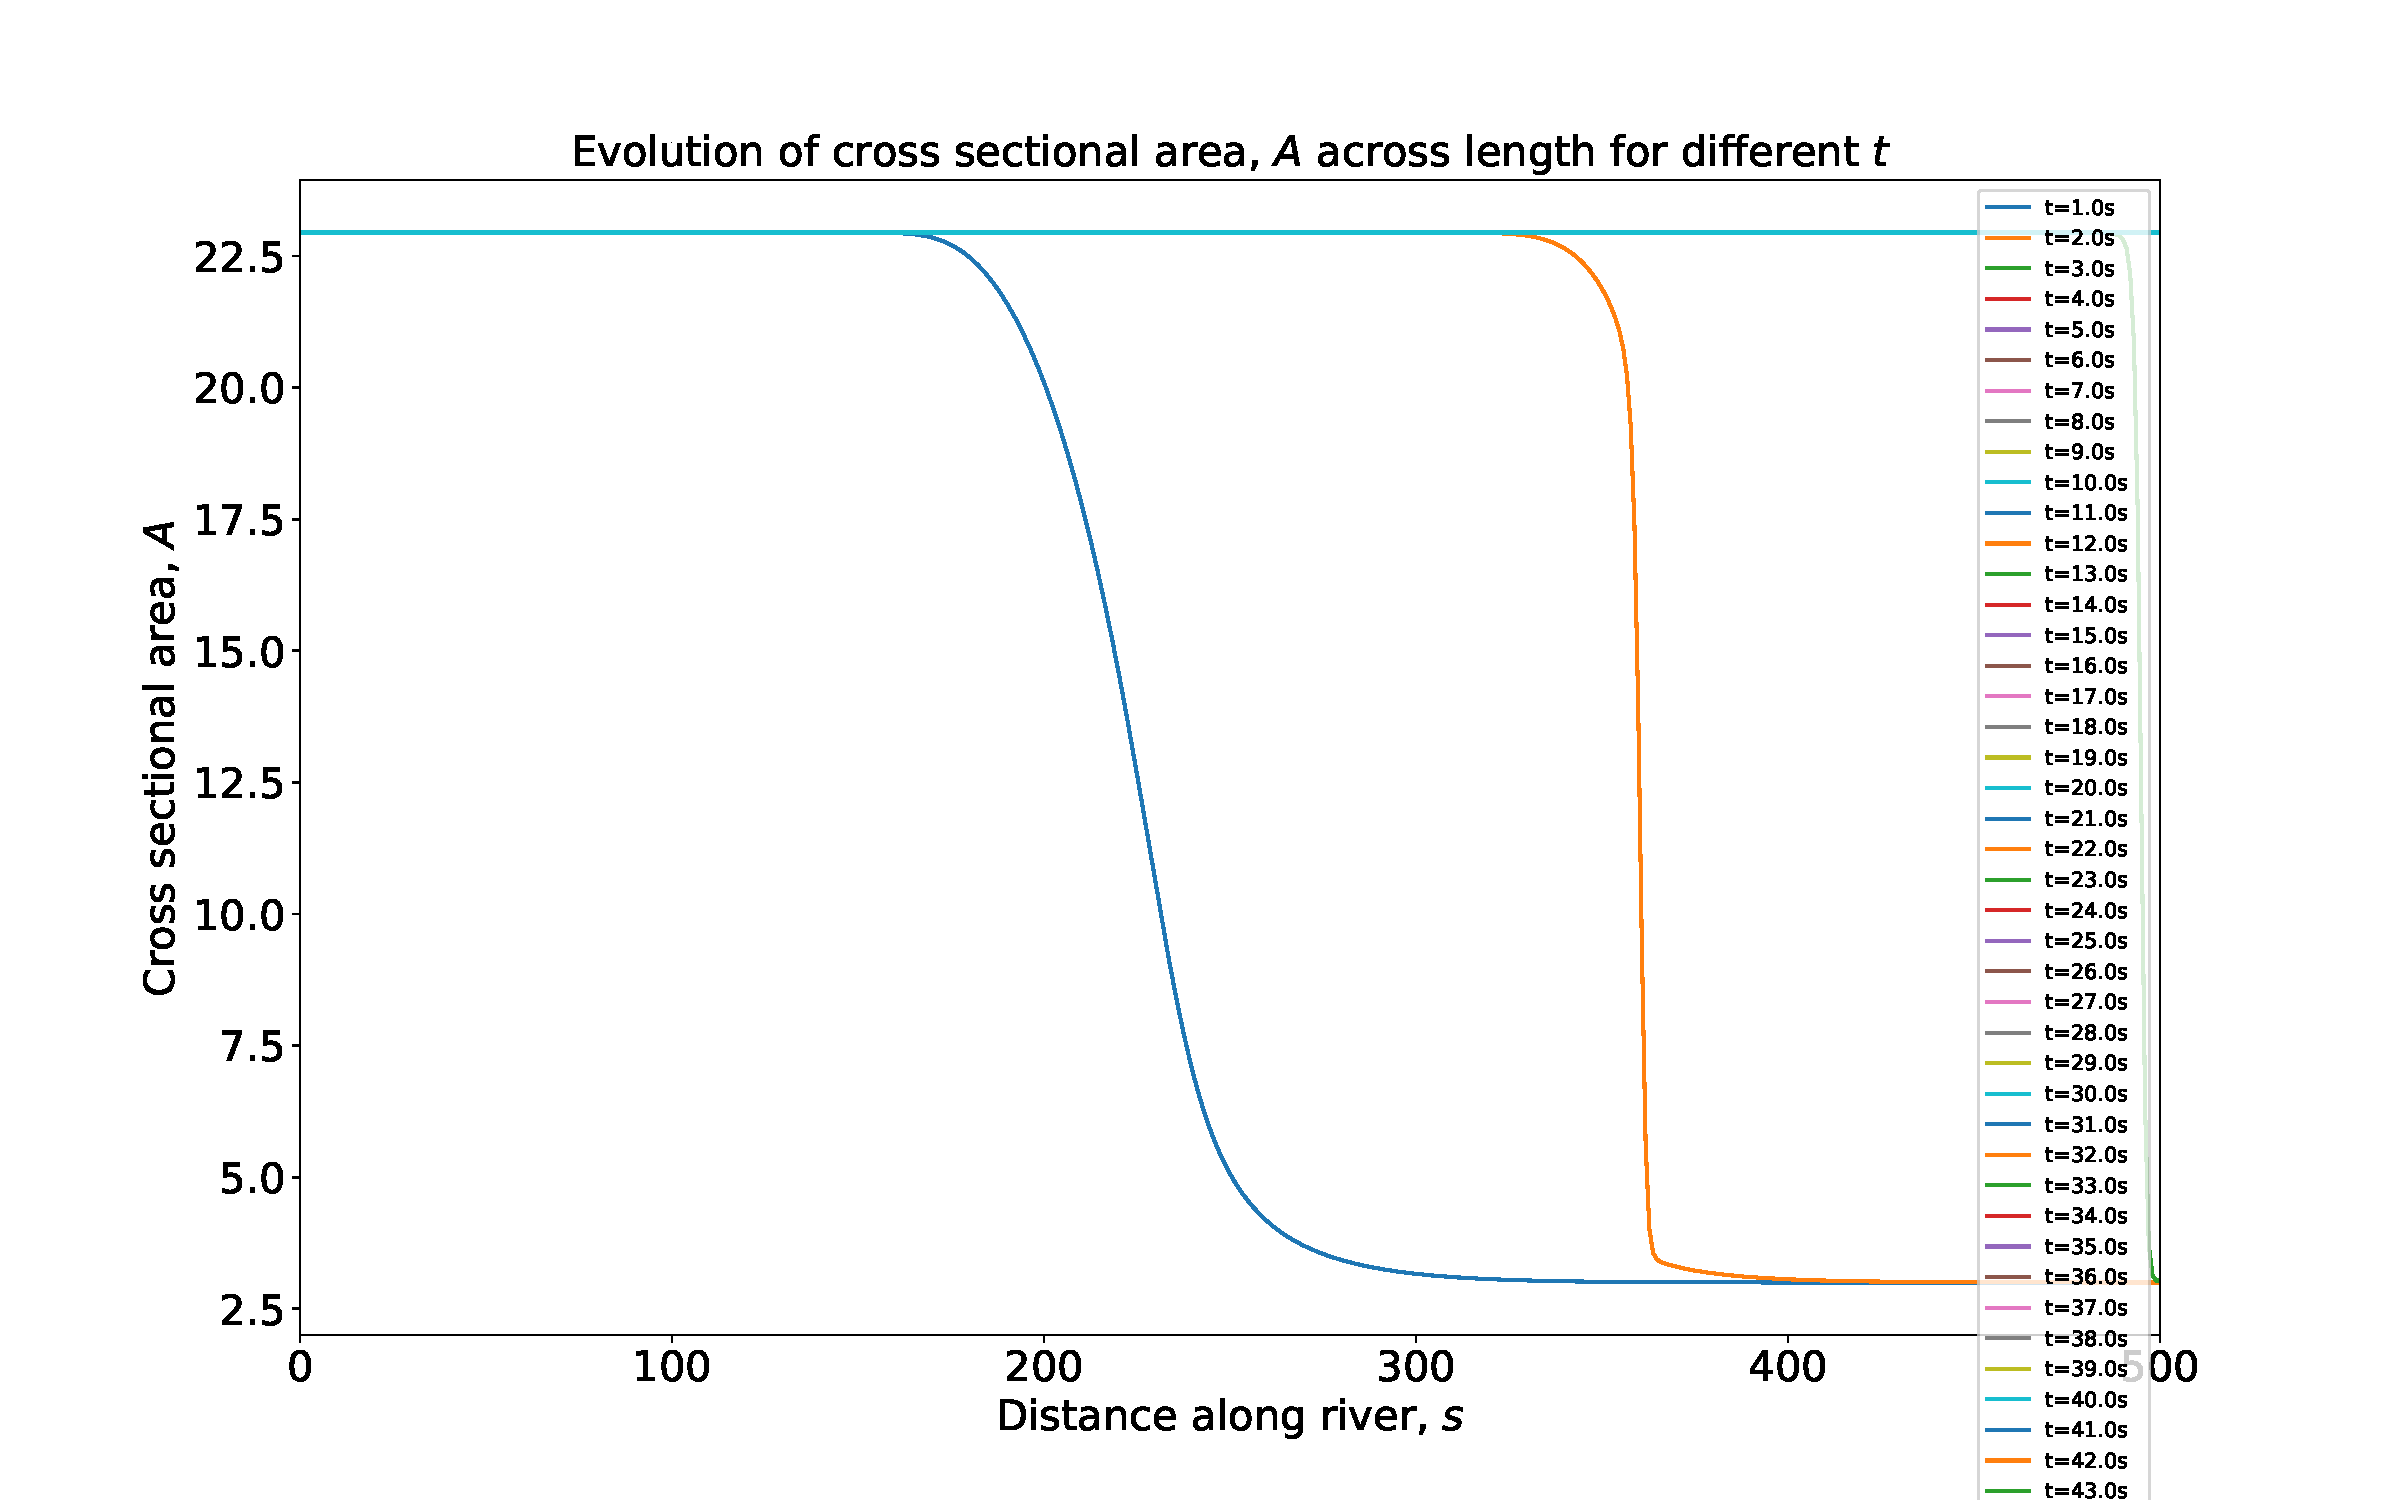
\includegraphics[width=\textwidth]{Figures/Rectangle_godunov.pdf}
        \caption{Visualisation of the Godunov method as a changing area, $A$ along the length of the river for different time $t$ for the rectangular cross section}
        \label{fig:rect_godunov}
    \end{subfigure}
    \caption{Plots regarding the rectangular channel. A shock forms at $t = $ and $s = $}
\end{figure}

In Fig. \ref{fig:wedge_char}, we notice that shock formation occurs at $s\approx 380\text{ m}$ and $t\approx 75\text{ s}$ with a calculated shock speed of $ 0.94\text{ ms}^{-1}$. However, according to Fig. \ref{fig:rect_godunov}.

\subsection{Wedge Channel}
For the wedge channel, the gradient percentage is at a higher value at $4-10\%$ (value taken is the median at $6.5\%$). To make the wedge comparable to the rectangular channel, we can set the variables to be $\theta = \pi$, have a comparable shape to the rectangle. We obtain $l =\sqrt{\frac{2A}{\left(\theta - \sin\theta\right)}}\theta$ and $l'(A) =\frac{2}{\sqrt{2A\sin(\theta)}}$.(See Appendix \ref{appendix:wedge} for detailed derivation.)

\begin{figure}[ht]
    \centering
    \begin{subfigure}[b]{0.49\textwidth}
        \centering
        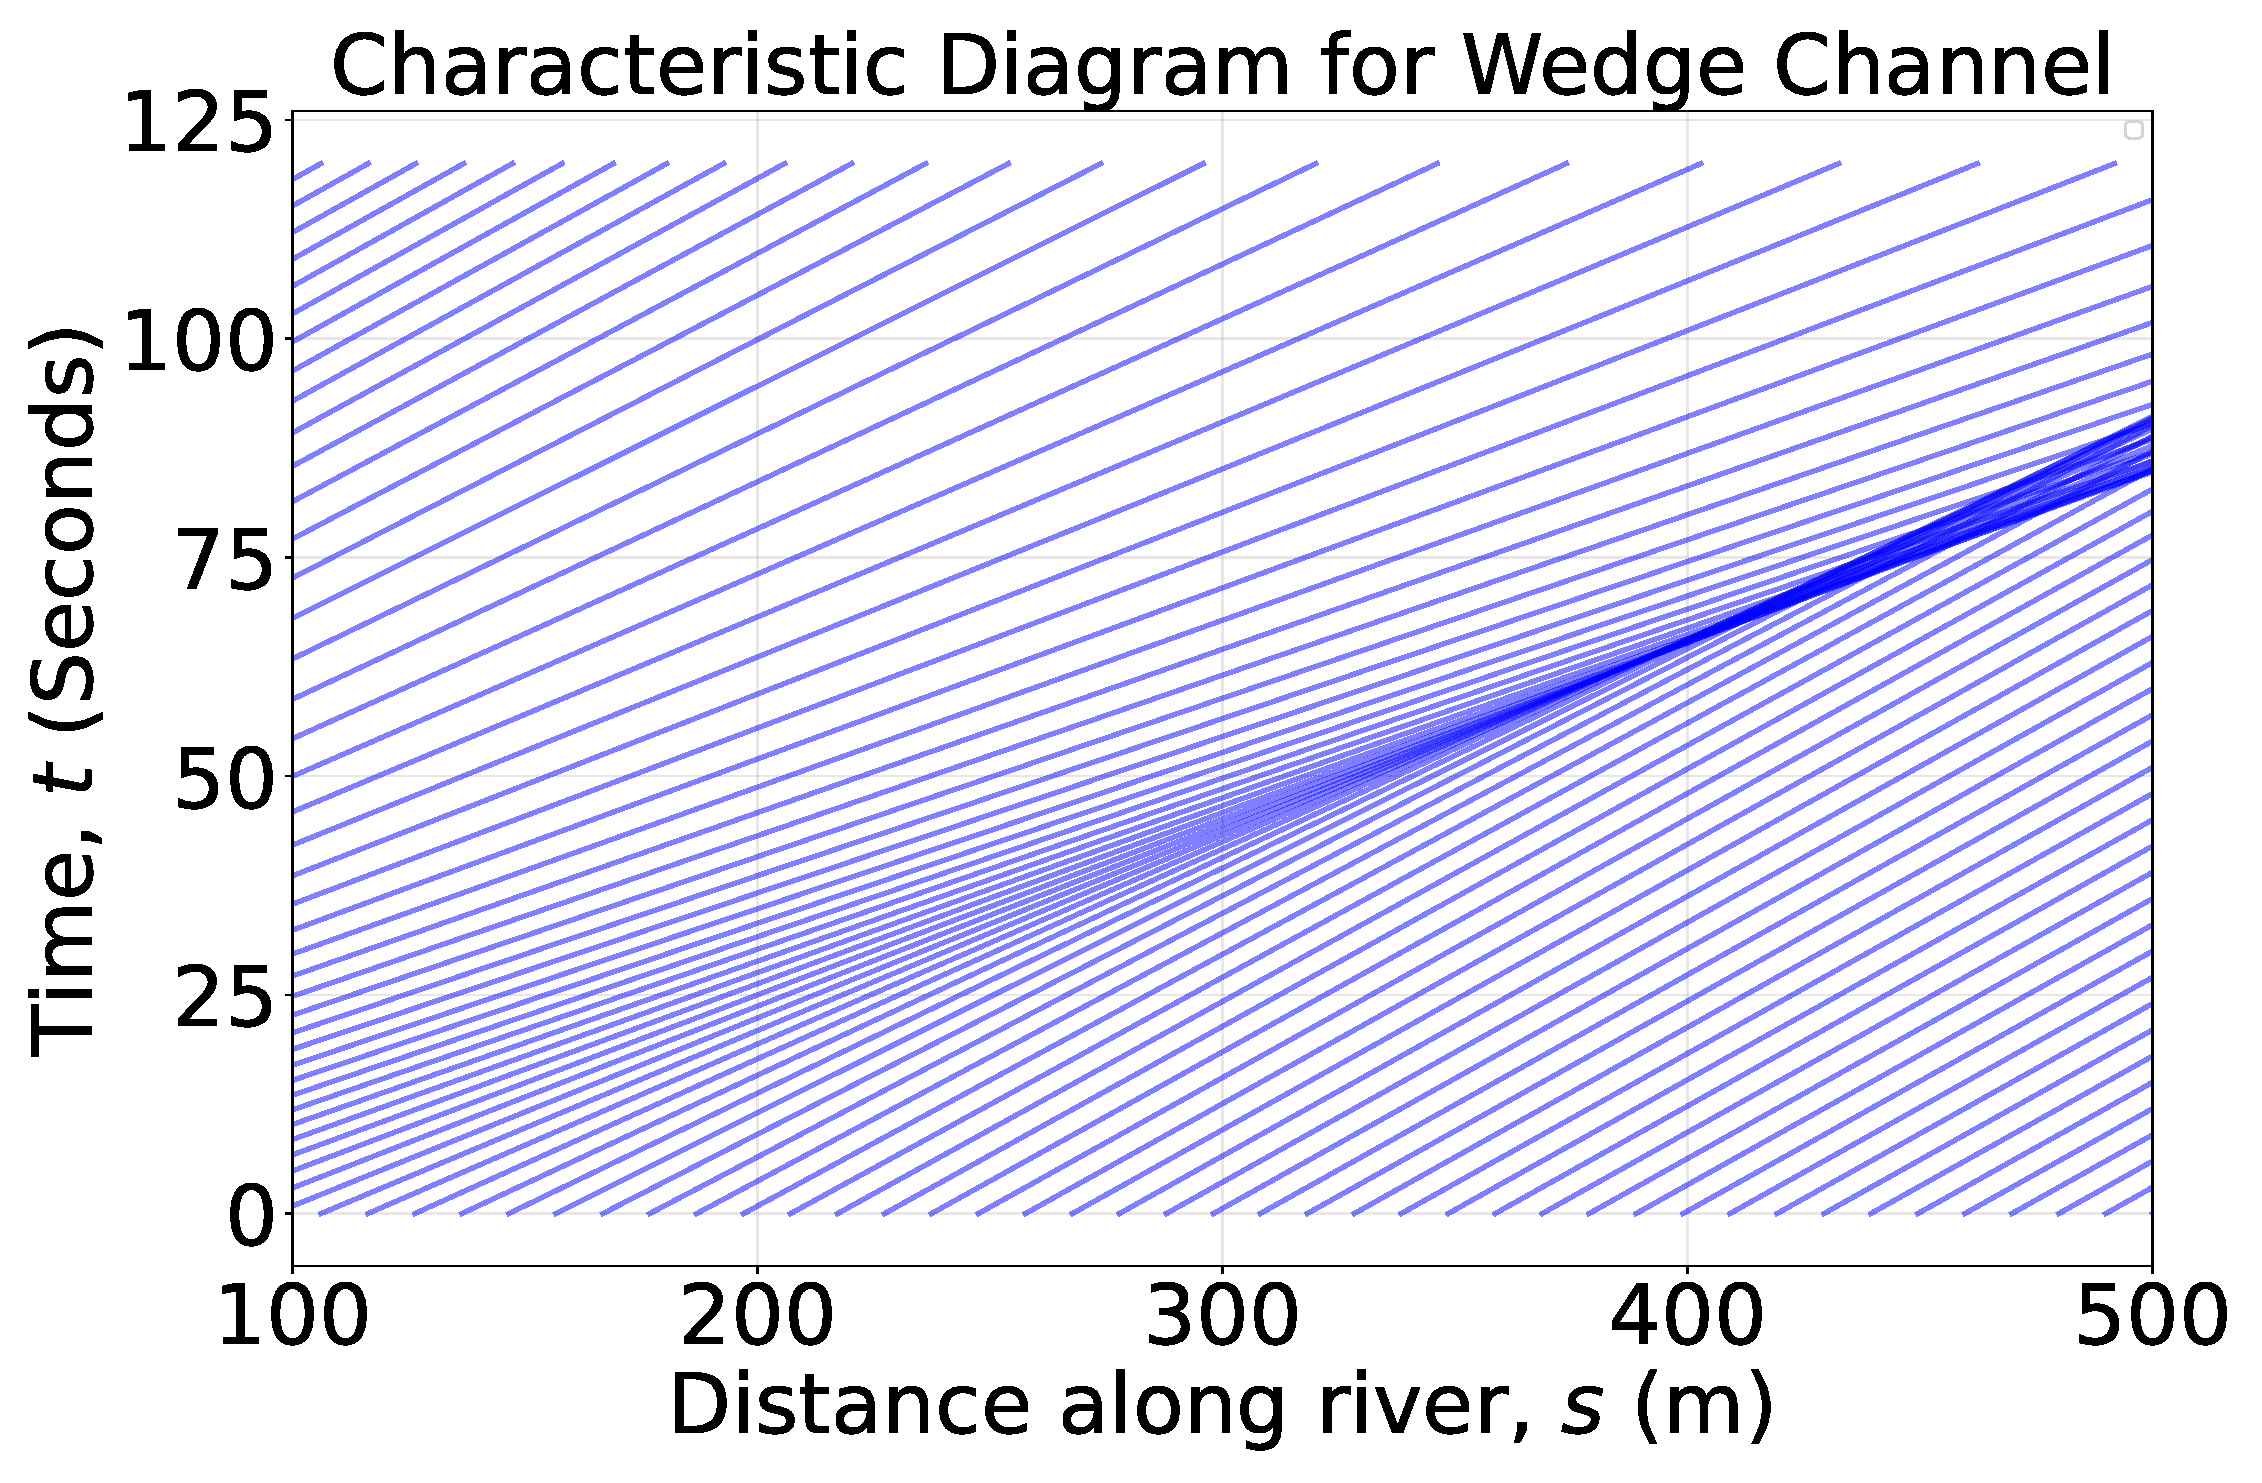
\includegraphics[width=\textwidth]{Figures/Wedge_characteristic.pdf}
        \caption{Characteristic equations for the wedge cross sections}
        \label{fig:wedge_char}
    \end{subfigure}
    \hfill
    \begin{subfigure}[b]{0.49\textwidth}
        \centering
        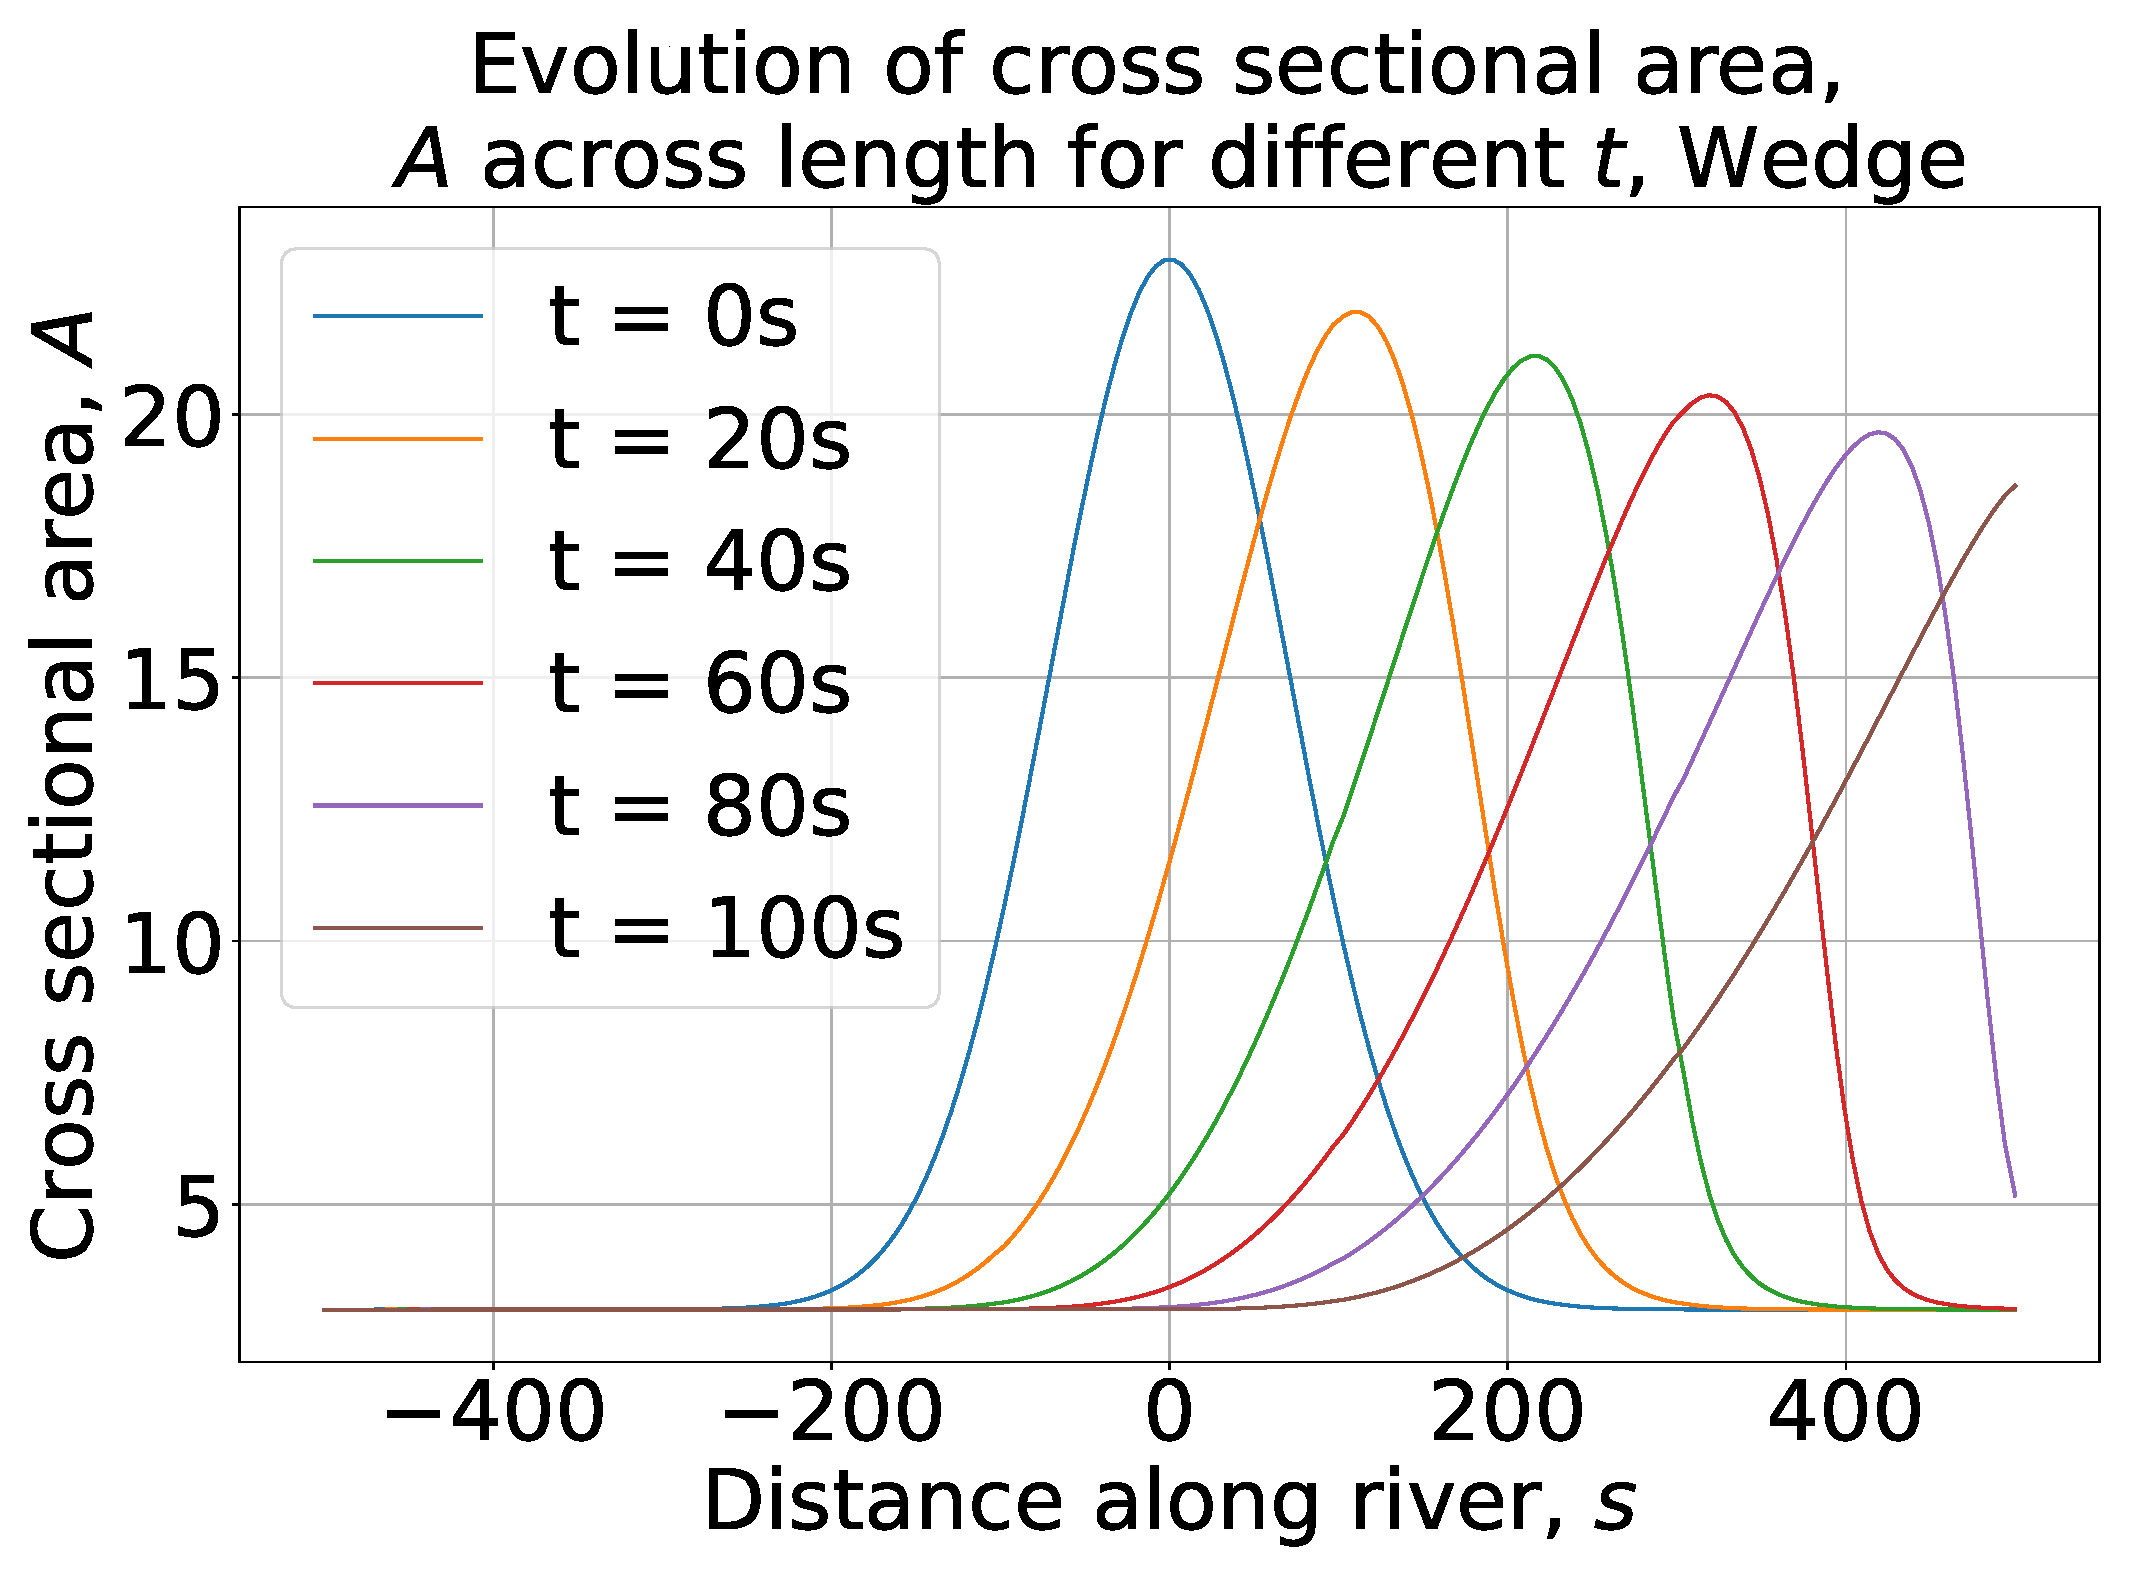
\includegraphics[width=\textwidth]{Figures/Wedge_godunov.pdf}
        \caption{Visualisation of the Godunov method as a changing area, $A$ along the length of the river for different times $t$ for the wedge cross section}
        \label{fig:wedge_godunov}
    \end{subfigure}
    \caption{Plots regarding the wedge channel. A shock forms at $t = $ and $s = $}
\end{figure}

In Figure \ref{fig:wedge_char}, we notice that shock formation occurs at $s= 420\text{ m}$ and $t= 60\text{ s}$, with a calculated shock speed of $ 4.1\text{ ms}^{-1}$, but showing a shock speed of $ \text{ ms}^-1$ in Fig. \ref{fig:wedge_godunov}.

\subsection{Semi-Circular}
Semi-circular - For a semi circular cross section that has a radius $R$ and $\theta$ is the central angle subtended by the water surface (Fig. \ref{fig:cross-sections}), $A = \frac{R^2}{2}\left(\theta - \sin\theta\right)$, $l = \sqrt{\frac{2A}{\left(\theta - \sin\theta\right)}}\theta$. $\alpha = 3\%$ and $\theta = \pi/3$. See Appendix \ref{appendix:semi-circular} for detailed derivation.

\begin{figure}[ht]
    \centering
    \begin{subfigure}[b]{0.49\textwidth}
        \centering
        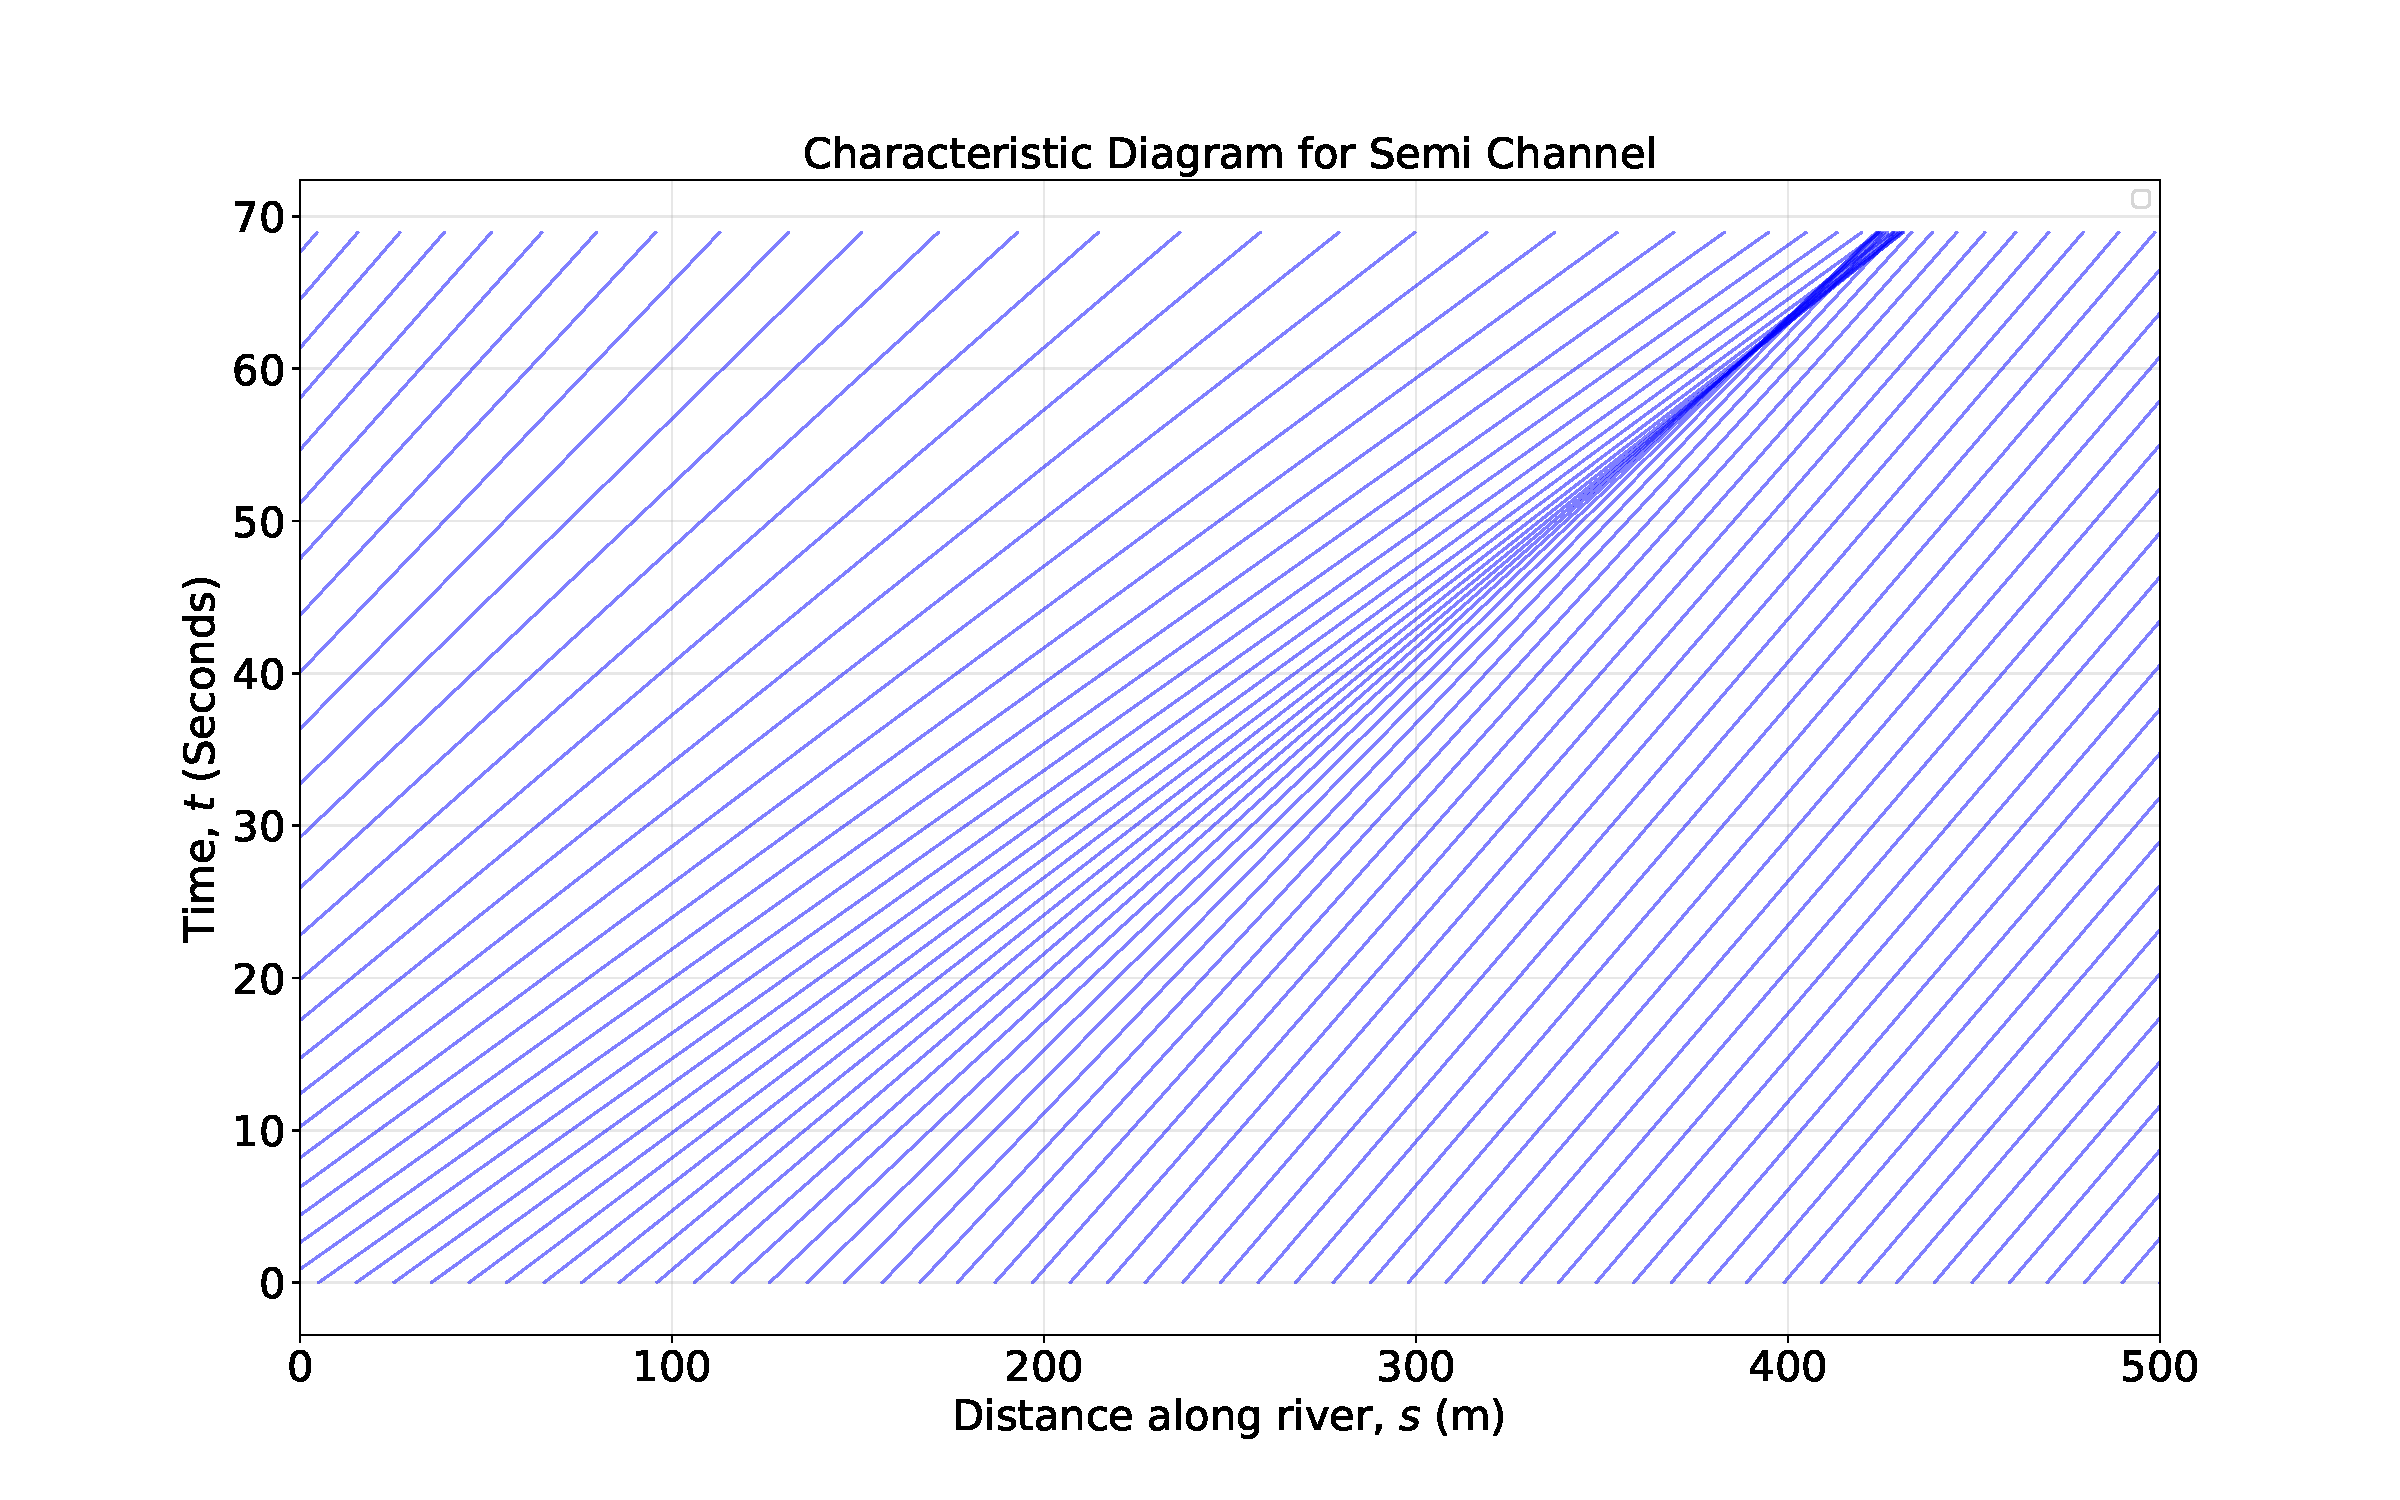
\includegraphics[width=\textwidth]{Figures/Semi_characteristic.pdf}
        \caption{Characteristic equations for the semicircular cross sections}
        \label{fig:semi_char}
    \end{subfigure}
    \hfill
    \begin{subfigure}[b]{0.49\textwidth}
        \centering
        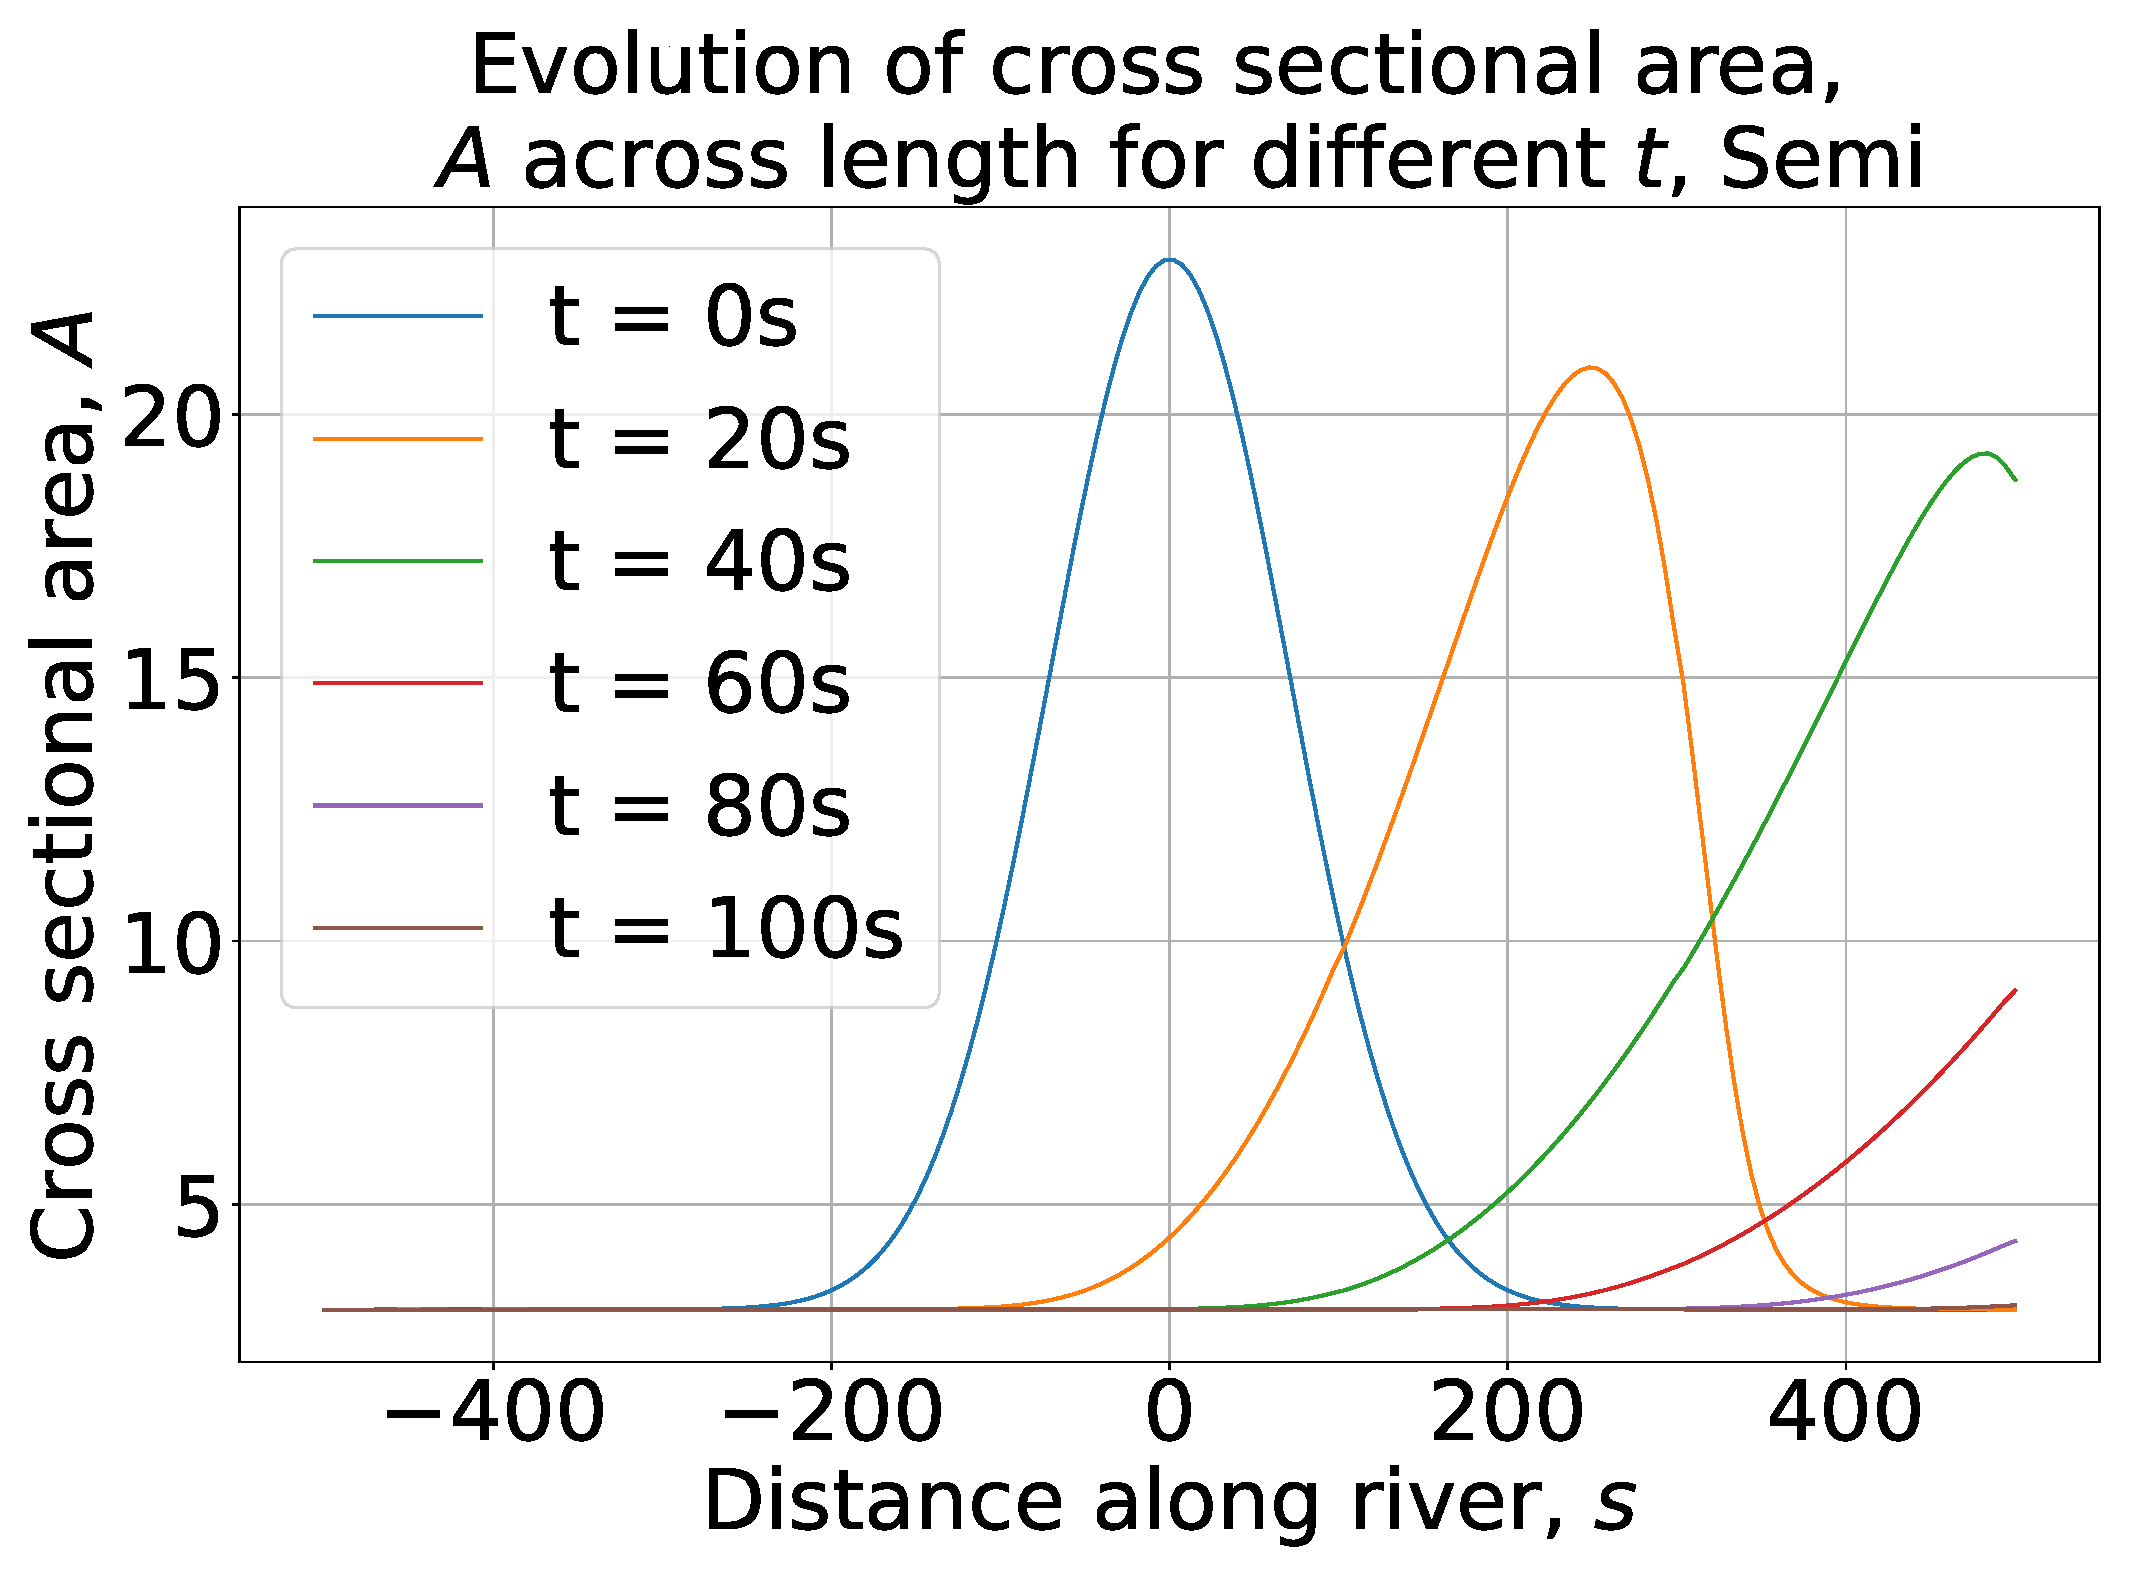
\includegraphics[width=\textwidth]{Figures/Semi_godunov.pdf}
        \caption{Visualisation of the Godunov method as a changing area, $A$ along the length of the river for different times $t$ for the semicircular cross section}
        \label{fig:semi_godunov}
    \end{subfigure}
    \caption{Plots regarding the wedge channel. A shock forms at $s= 400\text{ m}$ and $t= 80\text{ s}$}
\end{figure}

In Figure \ref{fig:wedge_char}, we notice that shock formation occurs at $s= 400\text{ m}$ and $t= 80\text{ s}$, with a calculated shock speed of $ 9.29\text{ ms}^{-1}$. In Fig. \ref{fig:wedge_godunov} there is indication of shock occurence at about $s\approx 400\text{ m}$ at $A = 25 \text{ m}^2$ however with a wrong value of $t$. This is the fastest out of the 3 cross sections in terms of the shock velocity. This means that water is easily expelled via a semi-circular cross section.

\subsection{Parabola}
Due to page count limit, the case of the parabola will not be investigated. However, the derivation of the perimeter $l(A)$ and $l'(A)$ can be found in Appendix \ref{appendix:parabola}. (As it would be a shame if all that math went to waste.)
\section{Conclusion}
% and further work
\newpage
\bibliographystyle{plain}
\bibliography{references}

\newpage
\appendix
\section{Derivation of areas and perimeters of cross-sections}
\subsection{Rectangle}
\label{appendix:rectangle}
For the rectangular channel of width $w$ and height of water $h$ (Fig. \ref{fig:cross-sections}(b)), the area and perimeter respectively are:
\begin{equation}
    \begin{split}
        A &= wh
        \\\text{Perimeter}&=2h + w
        \\l(A) &= w + \frac{2A}{w}
        \\\implies l'(A) &= \frac{2}{w}
    \end{split}
\end{equation}

\subsection{Wedge}
\label{appendix:wedge}
For a wedge (triangle) shaped cross section (Fig. \ref{fig:cross-sections}(c)) with sides $a$ and $b$ respectively, where $a = b$,
\begin{align}
    A &= \frac{1}{2}ab\sin(C) \notag
    \\&a = b = \frac{1}{2}l \notag
    \\A &= \frac{1}{8}l^2\sin{\theta}
\end{align}
With a perimeter of 
\begin{equation}
    l(A) = \sqrt{\frac{8A}{\sin{\theta}}}
\end{equation}

Giving a first order derivative:
\begin{equation}
    \begin{split}
          l'(A) &= \frac{1}{2}\frac{8}{\sin(\theta)}\left(\frac{8A}{\sin(\theta)}\right)^{1/2}
          \\&=\frac{4}{\sin(\theta)}\sqrt{\frac{8A}{\sin(\theta)}}
          \\&=\frac{2}{\sqrt{2A\sin(\theta)}}
    \end{split}
\end{equation}

\subsection{Semi-circular}
\label{appendix:semi-circular}
For a semi circular cross section (Fig. \ref{fig:cross-sections}(a)) that has a radius $R$ and $\theta$ is the central angle subtended by the water surface. We need to consider an expression for cases where the water is not completely full. As the water falls below the top of the river surface, a triangle is formed, which the area can be obtained by:
\begin{equation}
    A = \frac{R^2}{2} \sin\theta
\end{equation}

Therefore, the area of the cross section of water is:
\begin{align}
    A &=\frac{R^2 \theta}{2} - \frac{R^2}{2}\sin\theta \\
      &= \frac{R^2}{2}\left(\theta - \sin\theta\right) \notag
\end{align}
And the perimeter can be easily obtained:
\begin{align}
    l =& R\theta \\
        =& \sqrt{\frac{2A}{\left(\theta - \sin\theta\right)}}\theta \notag
\end{align}

And the derivative of $l(A)$ with respect to $A$ is:
\begin{equation}
    \begin{split}
         l'(A) &= \frac{\frac{1}{2}\frac{2}{\theta-\sin{\theta}}}{\sqrt{\frac{2A}{\theta-\sin{\theta}}}}\theta
        \\&= \frac{\theta}{\sqrt{2A(\theta-\sin{\theta})}}
    \end{split}
\end{equation}

\subsection{Parabola}
\label{appendix:parabola}
We can model a parabolic cross section by using the simple formula $y = ax^2$ (Fig. \ref{fig:cross-sections}(d)). The arc length and area can be obtained using simple derivation methods.

For a parabola, the arc length can be obtained using:
\begin{equation}
    L(a) = \int_0^a\sqrt{1 + y'(x)^2}dx
\end{equation}

For a cross section of width $2w$, the height of water will be $y(w) = aw^2$, giving a cross sectional area of:
\begin{equation}
    \begin{split}
        A &= (2w)(aw^2) - 2a\int_0^w dx \cdot x^2
        \\ &=2aw^3 - \frac{2aw^3}{3}
        \\ &=\frac{4aw^3}{3}
    \end{split}
\end{equation}

and the arc length:
\begin{equation}
    \begin{split}
        l&=2\int_0^wdx\sqrt{1 + (2ax)^2}
        \\
        \\ &\text{substitute }u=2ax\text{, }du=2a\cdot dx
        \\&=\frac{1}{a}\int_0^{2aw}du\sqrt{1 + u^2}
        \\
        \\ &\text{substitute }u=\tan(\theta)\text{, }du=\sec^2(\theta)\cdot d\theta\text{ , }1 + \tan^2(\theta) = sec^2(\theta)
        \\&=\frac{1}{a}\int_{\arctan(0)}^{\arctan{(2aw)}} d\theta \cdot \sec^3(\theta)
        \\&=\frac{1}{a}\left[\frac{1}{2}\sec{x}\tan{x}\right]_{\arctan(0)}^{\arctan(2aw)}+ \frac{1}{2}\int_{\arctan(0)}^{\arctan(2aw)} dx\sec{x}
        \\&= \frac{1}{2a}\left[\sec{x}\tan{x} + \ln{|\sec(x)+\tan(x)|}\right]_{\arctan(0)}^{\arctan(2aw)}
        \\&= \frac{1}{2a}(\sec(\arctan(2aw))\tan(\arctan(2aw)) + \ln{|\sec(\arctan(2aw))+\tan(\arctan(2aw))|})
        \\&=\frac{1}{2a}(2aw\sqrt{1 + (2aw)^2}+ \ln{|\sqrt{1 + (2aw)^2} + 2aw|})
    \end{split}
\end{equation}
Knowing that:
\begin{equation}
    \begin{split}
         \int \sec^3(x)dx &= \int \sec^2(x)\sec(x)dx
         \\&=\sec(x)\tan(x)-\int\sec(x)(\sec^2(x)-1)dx
         \\&=\sec(x)\tan(x)-\int\sec^3(x)dx+\int\sec(x)dx
         \\&=\frac{1}{2}\left(\sec(x)\tan(x)+\ln{|\sec(x)+\tan(x)|}\right) + C
    \end{split}
\end{equation}
and
\begin{equation}
    \sec(\tan(x)) = \sqrt{1+x^2}
\end{equation}
Expressing the length in terms of the area, since:
\begin{equation}
    a = \frac{3A}{4w^3} \implies 2aw = \frac{3A}{2w^2}
\end{equation}

\begin{equation}
    l(A) = \frac{2w^3}{3A}\left[\frac{3A}{2w^2}\sqrt{1 + \left(\frac{3A}{2w^2}\right)^2}+\ln\left|\sqrt{1 + \left(\frac{3A}{2w^2}\right)^2} + \frac{3A}{2w^2}\right|\right]
\end{equation}

To have an easier time finding the derivative, one can express the equation above in the simple form:
\begin{equation}
    \alpha(\beta + \ln{\gamma}) = \alpha'(\beta + \ln(\gamma)) + \alpha\left(\beta' + \frac{\gamma'}{\gamma}\right)
\end{equation}
The expression for $\alpha'$ is easy to obtain,
\begin{equation}
    \alpha' = -\frac{2w^3}{3A^2}
\end{equation}
$\beta$ is in the form of $x\sqrt{1 + x^2}$, where the derivative is:
\begin{equation}
    \begin{split}
        f(x) &= x\sqrt{1 + x^2}
        \\
        f'(x) &= \frac{1 + 2x^2}{\sqrt{1 + x^2}}
    \end{split}
\end{equation}
Using $x = \frac{3A}{2w^2}$ and the chain rule $\frac{d\beta}{dA} = \frac{d\beta}{dx}\cdot\frac{dx}{dA}$, we can conclude:
\begin{equation}
    \beta' = \frac{1 + 2\left(\frac{3A}{2w^2}\right)^2}{\sqrt{1 + \left(\frac{3A}{2w^2}\right)^2}}\frac{3}{2w^2}
\end{equation}

The final part of the derivative:
\begin{equation}
    \begin{split}
        \gamma' &= \frac{1}{2}\left(1 + \left(\frac{3A}{2w^2}\right)^2\right)^{-1/2}\cdot2\left(\frac{3A}{2w^2}\right)\left(\frac{3}{2w^2}\right)
        \\&=\frac{9A}{4w^4\sqrt{1 + \left(\frac{3A}{2w^2}\right)^2}}
    \end{split}
\end{equation}
And the first order derivative of $l(A)$ for the parabola is:
\begin{equation}
    \begin{split}
        l'(A) &= -\frac{2w^3}{3A^2}\cdot l(A) +  \frac{2w^3}{3A}\left[\frac{1 + 2\left(\frac{3A}{2w^2}\right)^2}{\sqrt{1 + \left(\frac{3A}{2w^2}\right)^2}}\frac{3}{2w^2} +  \frac{9A}{4w^4\sqrt{1 + \left(\frac{3A}{2w^2}\right)^2}}\right]
    \end{split}
\end{equation}

\end{document}


